\PassOptionsToPackage{unicode=true}{hyperref} % options for packages loaded elsewhere
\PassOptionsToPackage{hyphens}{url}
%
\documentclass[]{article}
\usepackage{lmodern}
\usepackage{amssymb,amsmath}
\usepackage{ifxetex,ifluatex}
\usepackage{fixltx2e} % provides \textsubscript
\ifnum 0\ifxetex 1\fi\ifluatex 1\fi=0 % if pdftex
  \usepackage[T1]{fontenc}
  \usepackage[utf8]{inputenc}
  \usepackage{textcomp} % provides euro and other symbols
\else % if luatex or xelatex
  \usepackage{unicode-math}
  \defaultfontfeatures{Ligatures=TeX,Scale=MatchLowercase}
\fi
% use upquote if available, for straight quotes in verbatim environments
\IfFileExists{upquote.sty}{\usepackage{upquote}}{}
% use microtype if available
\IfFileExists{microtype.sty}{%
\usepackage[]{microtype}
\UseMicrotypeSet[protrusion]{basicmath} % disable protrusion for tt fonts
}{}
\IfFileExists{parskip.sty}{%
\usepackage{parskip}
}{% else
\setlength{\parindent}{0pt}
\setlength{\parskip}{6pt plus 2pt minus 1pt}
}
\usepackage{hyperref}
\hypersetup{
            pdftitle={The Purchasing Power Parity Puzzle},
            pdfauthor={Fernando Agustin Falbo; Devashish Kumar; Daniela Leitch Barra},
            pdfborder={0 0 0},
            breaklinks=true}
\urlstyle{same}  % don't use monospace font for urls
\usepackage[margin=1in]{geometry}
\usepackage{longtable,booktabs}
% Fix footnotes in tables (requires footnote package)
\IfFileExists{footnote.sty}{\usepackage{footnote}\makesavenoteenv{longtable}}{}
\usepackage{graphicx,grffile}
\makeatletter
\def\maxwidth{\ifdim\Gin@nat@width>\linewidth\linewidth\else\Gin@nat@width\fi}
\def\maxheight{\ifdim\Gin@nat@height>\textheight\textheight\else\Gin@nat@height\fi}
\makeatother
% Scale images if necessary, so that they will not overflow the page
% margins by default, and it is still possible to overwrite the defaults
% using explicit options in \includegraphics[width, height, ...]{}
\setkeys{Gin}{width=\maxwidth,height=\maxheight,keepaspectratio}
\setlength{\emergencystretch}{3em}  % prevent overfull lines
\providecommand{\tightlist}{%
  \setlength{\itemsep}{0pt}\setlength{\parskip}{0pt}}
\setcounter{secnumdepth}{5}
% Redefines (sub)paragraphs to behave more like sections
\ifx\paragraph\undefined\else
\let\oldparagraph\paragraph
\renewcommand{\paragraph}[1]{\oldparagraph{#1}\mbox{}}
\fi
\ifx\subparagraph\undefined\else
\let\oldsubparagraph\subparagraph
\renewcommand{\subparagraph}[1]{\oldsubparagraph{#1}\mbox{}}
\fi

% set default figure placement to htbp
\makeatletter
\def\fps@figure{htbp}
\makeatother

\usepackage{floatrow}
\floatsetup[figure]{capposition=top}
\floatsetup[table]{capposition=top}
\floatplacement{figure}{H}
\floatplacement{table}{H}
\usepackage{pgfplots}
\usepackage{booktabs}
\usepackage{longtable}
\usepackage{array}
\usepackage{multirow}
\usepackage{wrapfig}
\usepackage{float}
\usepackage{colortbl}
\usepackage{pdflscape}
\usepackage{tabu}
\usepackage{threeparttable}
\usepackage{threeparttablex}
\usepackage[normalem]{ulem}
\usepackage{makecell}
\usepackage{xcolor}

\title{The Purchasing Power Parity Puzzle}
\author{Fernando Agustin Falbo \and Devashish Kumar \and Daniela Leitch Barra}
\date{May 2018}

\begin{document}
\maketitle
\begin{abstract}
Based in the Law of One Price, the basic theory concept underlying the Purchasing Power Parity is the convergence of the price levels of two countries under a common currency, however, despite its simplicity, it has been focus of strong debate sin the 1970's. Despite how natural the mean reversal sounds, the difficulty to prove its convergence to a stationary mean has not only posed doubts over the validity of the own concept of PPP, but also over famous econometric methods, such as the unit root and cointegrartion methods. The low power of these tests has surged as a strong hypothesis, reason for what some econometricians have opted to try new methods, the most relevant, the panel data methods. The purpose of this paper is make explicit the difference of those methods in the particular context of the Purchasing Power Parity, by replicating two important papers in the field and comparing the results obtained.
\end{abstract}

\hypertarget{introduction}{%
\section{Introduction}\label{introduction}}

Usually defined as an extremely simple concept, Purchasing Power Parity Puzzle (PPP)
is also a challenging one and has been focus of strong debates specially since the 1970's.
Based in the Law of One Price, the basic theory concept underlying the PPP is the
convergence of the price levels of two countries under a common currency, in other words,
as defined by Taylor A. and Taylor M. (2004):

\begin{quote}
\emph{``The nominal exchange rate between two currencies should be equal to the ratio of aggregate price levels between the two countries\ldots{}''}\\
\textbf{Taylor A. and Taylor M. (2004)}
\end{quote}

At a first sight this convergence might seem natural, however, when testing for stationarity, the results are ambiguous rising doubts about its validity, and also, over the validity of the traditional stationarity tests such as the unit root test and the cointegration method. In many cases, the random walk hypothesis couldn't be rejected.

Along different studies, results differ substantially when the measured period of time is changed and also the tests depend extremely on the size of the sample. For studies measuring the post-war period before 1973, the so-called Bretton Woods period, results suggest the stationarity of the PPP or a long-run mean reversal. However, the results radically change when current float years (post 1973) are taken, showing a PPP that never
converges to the initial mean after a shock. Also, in the cases where PPP followed a mean reversal, the sample sizes were mostly 100 years or greater (for example, Taylor and Lothian (1996) use 200 years of data), while as with smaller samples the validity of the PPP couldn't be proved, meaning that it was not possible to reject the random walk hypothesis. In this view, Abuaf and Jorion (1990) and Lothian and Taylor (1996), among others, reach the conclusion that, shocks to the exchange rates last an average of 3 years, therefore, convergence of PPP happens only in the long-run.

Among the reasons argued to explain the failure to reject the random walk hypothesis, it is possible to cite 2 that seem the most likely: (1) The low statistical power that unit root tests have, which implies that the sample sizes must be fairly big to obtain significant
results, and PPP is known for its slow convergence. (2) The mean that the PPP should converge to, is changing over time.

Fortunately, with the time, new methods have been applied to test for stationarity, specifically cointegration and panel data. These methods, especially panel data, have proved to have a stronger statistical power, which is very useful, in particular for testing
data after 1973, which is more scarce.

The focus of our work is on the replication of two important papers in the field: Mark Taylor's 1988 paper,``An empirical examination of long-run purchasing power parity using cointegration techniques'', and Jyh-Lin Wu and Shaowen Wu's 2001 work, ``Is Purchasing
Power Parity Overvalued?''.

While the title of the first gives an explicit description of what the paper is about, the Wu and Wu paper is less obvious. They explore panel data methods as means to test the stationarity of the PPP, which should require less years, given that the application of cross
sectional data provides more observations and enlarges the sample.

It is implicit that the focus of this work is mostly empirical and econometric. By replicating these papers and adding some extensions to them in terms of data to cover the most recent years, we pretend to show the methodological and outcome differences of each
method.

The paper is structured as follows: Section II provides a brief summary of the most relevant literature in PPP theory, Section III includes the Taylor paper replication and an extension of Taylor for the years 1988 to 1998. Section IV deals with the Wu and Wu unit
root replication, while Section V shows the panel data replication and Section VII closes our work with some conclusions.

\hypertarget{literature}{%
\section{Literature}\label{literature}}

Even though the concept of Purchasing Power Parity got important attention after World War I, it is a far more older concept. Proposed first by scholars of the Salamanca 2school in the XVI century (Rogoff 1996), PPP was not a widely known concept until Gustav Cassel proposed its use as means to set relative gold parities in order to start restoring the destroyed post-war economy (Rogoff 1996).

During the 1950's until the early 1990's many authors tried to construct absolute measures for the PPP. Here, the most relevant work came from Summers and Heston in 1991,in the work that concluded with the creation of the Penn World Table 5, a fairly exhaustive work that complied hundreds of prices for identical goods sold in participant countries. From the data obtained, a comparison of prices can be made and, by converting all prices to a same currency, the authors manage to get real quantity comparisons, thus, estimates of the PPP can also be obtained from there.

However, in the late 1970's and early 1980's, many studies trying to prove the convergence of the PPP using both, unit root and cointegration, weren't be able to reject therandom walk hypothesis, which eventually rose many doubts about the validity of the PPP.

Adler and Lehmann (1983) pose strong questions on the actual convergence of the PPP, even in the long-run, proposing that, instead of a mean reversal tendency what really exists is just a Martingale Behavior 1 . They argue that the long time that takes to the Real
Exchange Rate to get back to its mean when there is a shock, causes shocks to accumulate.

Overall, they propose that PPP is not valid neither in the short run nor in the long run. Most of the literature has used the Augmented Dickey-Fuller test to test for the presence of unit roots and, since the mid-seventies, the Phillips-Perron test has also been included
along with the ADF test in order to correct for serial correlation and heteroskedasticity in the error terms non-parametrically. However, these tests have been questioned for their low-power specially among relatively small samples, specially for years after 1973 where
the floating rate regime was adopted. The main argument is the low power of the general test explained previously. This hypothesis was tested by Perron (1989) where he proposes a ``crash model''. Despite the critics, Abuaf and Jorion (1990) and Taylor and Lothian (1996) reach the rejection of the unit root hypothesis, by the use of large sets of data.

In cointegration techniques, developed and popularized by Engel and Granger (1987), the results are also ambiguous, while Taylor (1988) cannot find convergence, Kugler and Lenz (1993) find mixed results, being unable to reject the random walk hypothesis for
Canada and the United States.

The newest methodology is panel data, and here the evidence in favor of the PPP is more robust. Wu (1996) and Oh (1996) largely reject the random walk hypothesis and Frankel and Rose (1995) also manage to prove PPP, even with data coming only after 1973. Wu and Wu (2001), one of our core papers, also largely rejects the non-stationarity hypothesis. Nevertheless, Hakkio (1986), and several other authors, present theoretical
evidence against the PPP hypothesis for data taken during the 1970's, therefore the theory \footnote{Martingale Behavior is when the expected value of a price in a future period, conditional on the prices of previous periods, yields the value of the current price} of PPP remains without a conclusive result.

\hypertarget{replication-of-taylor-1988}{%
\section{Replication of Taylor 1988}\label{replication-of-taylor-1988}}

Mark Taylor in the paper ``An empirical examination of long-run purchasing power parity using cointegration techniques'' (1988) applies the work of Engle and Granger (1987) on cointegration techniques to test PPP theory.

``If each element of a vector of time series \(x_t\) first achieves stationarity after differencing, but a linear combination \(\alpha ' x_t\) is already stationary, the time series \(x_t\) are said to be co-integrated with co-integrating vector \(\alpha\)'' (Engle \(\&\) Granger, 1987, p.~251). Engle and Granger proposed the cointegration method as a broad tool to study any equilibrium relationships where related variables can diverge but will exhibit a tendency to converge back to equilibrium with finite expected time. In other words, cointegration tests for stationary of \(z_t\) where \(z_t = \alpha ' x_t\).

Taylor used this method to test PPP where the relevant two variables are \(e_t\), the logarithm of nominal exchange rate at time \(t\) (in terms of domestic price of foreign currency), and \(p_t\), the logarithm of the ratio of domestic to foreign price level at time \(t\). Previous studies mentioned by Taylor, such as Rogalski and Vinso (1977) and Roll (1979) used \(c_t = e_t - p_t\), and tested for stationarity of \(c_t\).

These studies failed to reject the null hypothesis that PPP deviations follow a random walk by testing for unit root in the \(c_t\) process. Taylor instead uses \(g_t\), where \(g_t = e_t - \alpha p_t\). \(g_t\) differs from \(c_t\) only because of the \(\alpha\) term and thus is less stringent since \(g_t\) being stationary for some value of \(\alpha\) is a necessary condition for \(c_t\) to be stationary; after all \(c_t\) is simply a special case of \(g_t\) where \(\alpha = 1\).

Taylor argues that an \(\alpha\) value other than 1 can be used to allow for measurement errors (of inflation measures for example) and/or transportation costs. Thus, if cointegration techniques show a unit root in \(g_t\) it would support previous work showing PPP deviations are not stationary but ``the converse finding could clearly be most striking in that we would have explained previous rejections of long-run PPP in terms of measurement error and/or transportation cost'' (Taylor, 1988, p.~1371).

\hypertarget{cointegration-overview}{%
\subsection{Cointegration overview}\label{cointegration-overview}}

Engle and Granger (1987) and Taylor (1988) give a straightforward explanation of cointegration. First, a series \(x_t\) is said to be \(I(d)\) if after differencing \(d\) times the series is stationary.

If \(x_t\) and \(y_t\) are I(d) then \(z_t = x_t - \alpha y_t\) will generally be I(d). However, if \(z_t\) is I(d-b), \(b>0\), then \(x_t\) and \(y_t\) are said to be cointegrated or CI(\(d\),\(b\)). In particular, if \(x_t\) and \(y_t\) are I(1), then it implies that the series are not stationarity but when the first difference are taken we get stationary series in both cases. Typically any linear combination of \(x_t\) and \(y_t\) would be expected to be I(1) also; however, if there exists an \(\alpha\) such that \(x_t - \alpha y_t\) is stationary, or I(0) then we say \(x_t\) and \(y_t\) are said to be cointegrated or CI(1,1).

Also note that, if \(x_t\) and \(y_t\) are already I(0), then \(z_t\) will always be I(0) thus we need the series to be both I(1), at least.

We now replicate Taylor's cointegration test as follows: Test hypothesis that \(e_t\) and \(p_t\) are I(1) series. And citing Taylor himself:
\textgreater{} ``If we cannot reject this hypothesis, we can go on to test for cointegration by testing the residuals from the cointegrating regressions to see if they appear to be I(0). Only if we can reject the hypothesis that the cointegrating residuals are I(1) can we claim to have found cointegration, and hence a form of long-run PPP.''

\hypertarget{conclusions-from-taylors-cointegration-technique}{%
\subsection{Conclusions from Taylor's cointegration technique}\label{conclusions-from-taylors-cointegration-technique}}

Taylor's study ultimately was unable to reject the hypothesis of non-cointegration of exchange rate and relative prices, and thus, his study did not find support for PPP empirically. We reached the same conclusion using the data from the period that Taylor used (June 1973 to December 1985).

\begin{itemize}
\tightlist
\item
  Testing that nominal exchange rate are I(1)

  \begin{itemize}
  \tightlist
  \item
    Testing unit root of nominal exchange rate: For all five currencies considered we were unable to reject the null hypothesis of non-stationarity
  \item
    Testing unit root of first differences of nominal exchange rate: For all five currencies considered, we were unable to reject the null hypothesis of non-stationarity for nominal exchange rate (or more precisely logarithm of the nominal exchange rate). Then, when first differences were tested for unit-root we were able to reject the null hypothesis of non-stationarity. For a detailed description of results, see Table \ref{tab:ner} in the appendix.
  \end{itemize}
\item
  Testing for unit root in relative prices

  \begin{itemize}
  \tightlist
  \item
    Testing unit root of relative price level: Similar to Taylor's paper we were unable to reject the null hypothesis of non-stationarity for all currencies except one. The exception we found was Japan whereas the original paper found this to be the case for (West) Germany.
  \item
    Testing unit root of first differences of relative price level: First differences were tested for unit-root and we were able to reject the null hypothesis of non-stationarity for all countries. However, since for Japan (and West Germany in the case of the original paper) we could reject null-hypothesis of non-stationarity in the original series we can reject I(1) null-hypothesis for that country. However, for the other countries we are unable to reject the I(1) null hypothesis for the (logarithm) of relative price levels. Table \ref{tab:pl} presents our results.
  \end{itemize}
\item
  Cointegration test

  \begin{itemize}
  \tightlist
  \item
    For countries that we were unable to reject the I(1) hypothesis, we can now test for cointegration. Since for Japan our data suggests that currency level is I(1) but relative price level is I(0), we cannot have cointegration. However, similar to Taylor, we test for cointegration for all the countries including Japan for comparison purposes.
  \item
    We test for cointegration by testing the null hypothesis of non-stationarity in the cointegration regression residuals. In all cases, we fail to reject the null hypothesis thus we do not have evidence of cointegration (see Table \ref{tab:coin}).
  \end{itemize}
\end{itemize}

While our statistics do not match the exact numbers in the original number our conclusions are exactly the same. The paper was written more than thirty years ago and the data has been reindexed, and possibly upgraded. For example, there is no West Germany series available on the IMF website so we instead used the Germany data. Please also note that we used the exchange rate as foreign currency by USD which is the reciprocal of the definition used by the paper - this is the original format of the data available on IMF so we kept that as the format. (Thus the slope coefficients for the cointegration regression are negative instead of being positive).

\hypertarget{extension-of-taylor-test-to-more-periods}{%
\subsection{Extension of Taylor test to more periods}\label{extension-of-taylor-test-to-more-periods}}

We repeated the exercise above to include data until December 1998 on the same countries. We stopped in 1998 since data after that year assumes a single Euro currency. Using the augmented data, from May 1973 to December 1998, we still fail to reject the null hypothesis of non-stationarity in the cointegration regression residuals. The results for this extension are shown in Tables \ref{tab:ner2}, \ref{tab:pl2}, \ref{tab:coin2} in the appendix.These results are discouraging for believers of purchasing power parity.

\hypertarget{the-adf-and-panel-tests}{%
\section{The ADF and Panel Tests}\label{the-adf-and-panel-tests}}

\hypertarget{univariate-series-unit-roots-testadf}{%
\subsection{Univariate Series Unit Roots Test:ADF}\label{univariate-series-unit-roots-testadf}}

Consider the univariate time model process:

\begin{eqnarray*}
y_{t} =\theta y_{t-1} + \varepsilon_{t} & \textrm{, with} & \theta = 1 \\
(1-L)y_{t} = \varepsilon_{t}
\end{eqnarray*}

The process is a nonstationary AR(1) with one unit root. In other words, the variable \(y_{t}\) will not revert to a constant mean.
Note that the first difference is stationary:

\begin{align*}
\Delta y_{t} &= y_{t} - y_{t-1}\\
\Delta y_{t} &= \varepsilon_{t}
\end{align*}

In general, in a nonstationary process with \(k\) unit roots (or with \(k\) lags with coefficients equal one), the \(k\) difference will be stationary.

A Unit root test has the objective to detect unit roots in the data generating process. Basically, the main idea is to build a test with a null Hypothesis: \(H_{0} : \theta = 1\) (non-stationarity). On the other hand, \(H_{1}: \theta < 1\) (stationarity). If there is evidence to reject the null hypothesis, a stationary process could be concluded.

In the estimation for the AR(1) process, the standard t-statistic for the \(H_{0}\) hypothesis is given by:

\[DF = \dfrac{\hat{\theta} - 1}{se(\hat{\theta})}\]

The problem is that it has not the standard distribution under the null hypothesis. If \(\theta = 1\), \(Var[y_{t}]\) is not even defined, so a nonstationary process invalidates the results of the OLS estimation. As the critical values of the t-distribution cannot be used, the solution to this problem is to keep the test statistics, but using different critical values. The correct distribution for this test is provided by Dickey and Fuller (1979). Therefore, the test is known as \textbf{Dickey-Fuller Test}.
Note that if \(y_{t-1}\) is subtracted in both sides:

\[\Delta y_{t} = (\theta - 1)y_{t-1} + \varepsilon_{t}\]

The t-statistic for \((\theta - 1) = 0\) is identical to the \(DF\). The critical values will depend on the number of data and other model specifications (as a linear drift and constant terms). Consider the general case, where a linear trend and an intercept are included:

\[\Delta y_{t} = \alpha + \beta t + (\theta -1)y_{t-1} + \varepsilon_{t}\]

\[\textrm{Let's call} (\theta -1) = \rho\]

If the general model is considered for a general AR(p) process, we estimate the Augmented Dickey Fuller Test (\textbf{ADF}):

\[\Delta y_{t} = \alpha + \beta t + \rho y_{t-1} + \varPhi_1\Delta y_{t-1} + \dots + \varPhi_k\Delta y_{t-k} + \varepsilon_{t}\]

Where the null hypothesis is \(H_{0}: \rho = 0\), and the model must be specified beforehand the estimation (Constant, trend and number of lags).

\hypertarget{panel-unit-roots-test-ips-and-mw}{%
\subsection{Panel Unit Roots Test: IPS and MW}\label{panel-unit-roots-test-ips-and-mw}}

\begin{quote}
\emph{``The low power of unit root tests against highly persistent alternatives with anything less than a century of data has inspired the development of panel unit root tests which exploit cross-section, as well as time series, variation. Variants of these tests have been developed by Levin and Lin (1992) (LL), Im et al. (1997) (IPS), Maddala and Wu (1999), and Bowman (1999). Applications of these tests to post-1973 real exchange rates of industrialized countries include Abuaf and Jorion (1990), Frankel and Rose (1996), Jorion and Sweeney (1996), Oh (1996), Wu (1996), O'Connell (1998a, 1997), Papell and Theodoridis (1998, 2001), and Wu and Wu (2001). A panel extension of the univariate ADF test in previous section, which accounts for both a heterogeneous intercept and serial correlation, would involve estimating the following equations''}\\
\textbf{(Papell, 2001)}
\end{quote}

\begin{eqnarray*}
    y_{i,t} =\alpha_{i} + \rho_{i}q_{i, t-1} + \sum_{j=1}^{k_{j}}\Phi_{i,j}\Delta q_{i, t-j} + \varepsilon_{i,t}  & i = 1, \dots, N. 
\end{eqnarray*}

In the following paragraphs, we will explain with more details the IPS and the WM tests, which will be use in our replication for test PPP in a Panel Data Set.

\hypertarget{the-im-pesaran-shin-ips-test}{%
\subsection{The Im-Pesaran-Shin (IPS) Test}\label{the-im-pesaran-shin-ips-test}}

The following explanation was taken from Hoang \& Mcnown (2006):

We start with our model:

\begin{eqnarray*}
    y_{i,t} =\alpha_{i} \theta_{i} y_{i,t-1} + \varepsilon_{i,t} 
\end{eqnarray*}

With \(t = 1, 2, \dots, T\) and \(i = 1, 2, \dots, N\)

Null hypothesis is defined as: \(H_{0} = \theta_{i} = 1\), for \(i = 1, 2, \dots, N\)

And the alternative hypothesis is defined as: \(H_{0} = \theta_{i} < 1\) for \(i = 1, 2, \dots, N_{1}\), and \(\theta_{i} = 1\) for \(i = N_{1} + 1, N_{1} + 2, \dots, N\)

Note that while the null hypothesis states that all the series included have unit root, the alternative hypothesis states that some of the series included in the panel are stationary.
Using ADF tests for the N cross-section units, we get the t-statistic for each individual serie \(i\): \(t_{i,T}\). Assume that \(E[t_{i,T}] = \mu\) and \(Var[t_{i,t}] = \sigma^2\). Then:

\[\bar{t}_{N,T} = \frac{1}{N} \sum_{i=1}^{N}t_{i,t}\]

and

\[\sqrt{N}\frac{(\bar{t}_{N,T} - \mu)}{\sigma} \underset{N \rightarrow \infty}{\Longrightarrow} N(0,1)\]

Note that the IPS test is a standardized average of individual ADF statistics. The key assumption is that T does not change through cross-section units and therefore \(E[t_{i,T}]\) and \(Var[t_{i,T}]\) are the same for all i. Because of that, the IPS test can only be applied in balanced panel data.

\hypertarget{maddala-and-wu-mw-test}{%
\subsection{Maddala and Wu (MW) Test}\label{maddala-and-wu-mw-test}}

The following explanation was taken from Hoang \& Mcnown (2006):

\emph{``As in the IPS, we have to use the ADF estimation equation in each cross-section, but with a different transformation.''}

Taking the ADF t-statistic for each series we found the corresponding p-value from the empirical ADF distribution obtained through a Monte-Carlo simulation. Then we compute a Fisher-test statistics and compare it with the the appropriate \(\chi^2\) critical value.

Note that the Fisher's (\(p \lambda\)) test is based on the p-values combination of the test-statistic for a unit root in each cross-sectional individual.

Let \(\pi_{i}\) be the p-value from the ith-test such that \(\pi_{i}\) are \(U[0, 1]\) and independent, and \(-2log_{e}\pi_{i}\) has a \(\chi^2\)distribution with 2 degrees of freedom. So \(p \lambda = -2 \sum_{i=1}^{N} log \pi_i\) has a \(\chi^2\) distribution with \(2N\) degrees of freedom. The null and alternative hypotheses are the same as in the IPS test.

\hypertarget{replicating-wu-wu-test-ppp-with-adf-and-panel-tests}{%
\section{Replicating Wu \& Wu: Test PPP with ADF and Panel Tests}\label{replicating-wu-wu-test-ppp-with-adf-and-panel-tests}}

\hypertarget{model}{%
\subsection{Model}\label{model}}

In this section we use ADF and Panel tests on real exchange rates to replicate the 2001 paper \emph{``Is Purchasing Power Parity Overvalued?''} by Jyh-Lin Wu and Shaowen Wu. If we can reject the null hypothesis of nonstationarity, then PPP holds in the long run.

Let's define the real exchange rate \(Q\) as:

\[Q_{t} = \frac{E_{t}P^*_{t}}{P_{t}}\]

Where \(E\) is the nominal exchange rate (domestic currency per foreign currency), \(P^*\) is the price level in the foreign country and \(P\) is the price level in the domestic economy. In our model, we consider bilateral real exchange rates with United States (U.S.), so the nominal exchange rate is domestic currency per U.S. dollar and \(P^*\) is U.S. price levels.
Applying logs:

\[q_{t} = e_{t} + p^*_{t} - p_{t}\]

According to PPP Theory, real exchange rate \(q\) should tend to a constant value in the longer run. Permanent deviations are not allowed. This theory is based in the Law of One Price (LOP). For example, if the domestic prices increase, then exports will decrease and imports will rise, which will push the nominal exchange rate up to compensate the real exchange rate. This means that the real exchange rate should be stationary, in other words, it should have a constant mean and the variance should not depend on time.

\[q_{t} = \alpha + \theta q_{t-1} + \varepsilon_{t}\]

If PPP holds, \(|\theta| < 1\). Therefore, we can use ADF Tests to check \(\theta\) value for each country. Note that, as we have seen above, it is convenient to use the differenced transformed version. The model to estimate is the following:

\[\Delta q_{t} = \alpha + \beta t + \rho q_{t-1} + \varPhi_1\Delta q_{t-1} + \dots + \varPhi_k\Delta q_{t-k} + \varepsilon_{t}\]

Note that a time trend should not be included in the case of PPP testing, because that would be theoretically inconsistent with long-run PPP (Papell, 2001). The null hypothesis of a unit root is rejected in favor of the alternative of level stationarity if \(\rho\) is significantly different from zero.

Additionally, we can use Panel Unit Roots tests using the whole the sample (all countries and all time periods). Note that for N countries, we get:

\begin{eqnarray*}
    q_{i,t} =\alpha_{i} + \rho_{i}q_{i, t-1} + \sum_{j=1}^{k_{j}}\Phi_{i,j}\Delta q_{i, t-j} + \varepsilon_{i,t}  & i = 1, \dots, N. 
\end{eqnarray*}

\hypertarget{data}{%
\subsection{Data}\label{data}}

We used quarterly data for 20 developed countries \footnote{Australia, Austria, Belgium, Canada, Denmark, Finland, France, Germany, Greece, Ireland, Italy, Japan, the Netherlands, New Zealand, Norway, Portugal, Spain, Sweden, Switzerland, and the United Kingdom} from 1973-Q2 to 1997-Q4. The source is the International Monetary Fund's International Financial Statistics. We used the Consumer Price Index (CPI) as the price level for each country.

For the Panel Tests, we also used subsamples: The European Community (EC), The European Monetary System (EMS), the Group of 6 (G6)\footnote{Canada, France, Germany, Italy, Japan and the United Kingdom}, and the Group of 10 (G10)\footnote{Belgium, Canada, France, Germany, Italy, Japan, the Netherlands, Sweden, Switzerland, and the United Kingdom}.

\begin{figure}

{\centering 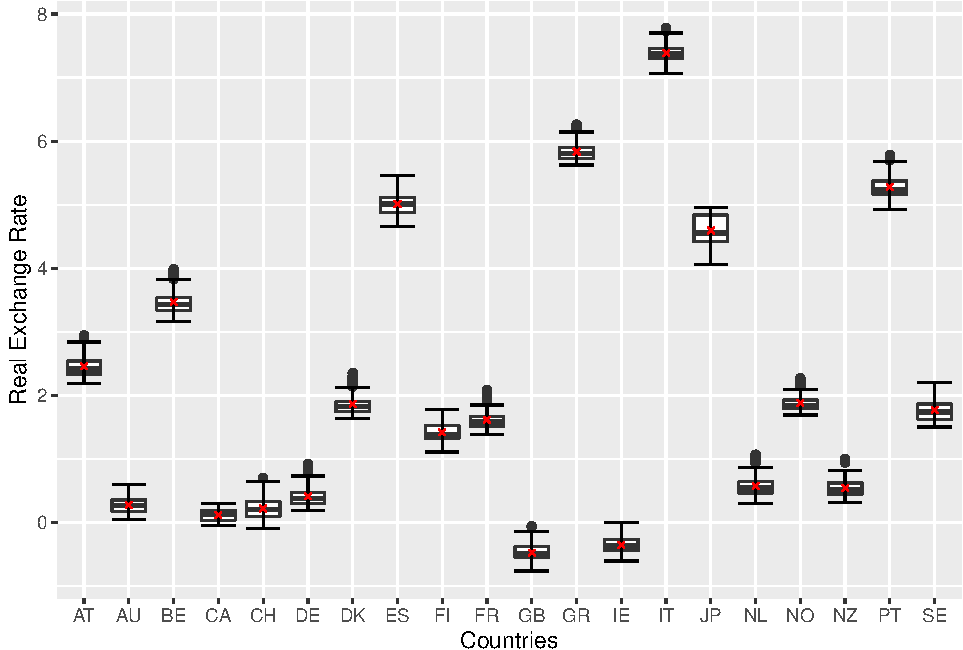
\includegraphics[width=0.75\linewidth]{Time_Series_v_pdf_files/figure-latex/rer1-1} 

}

\caption{Average Country Real Exchange Rate}\label{fig:rer1}
\end{figure}

\begin{figure}

{\centering 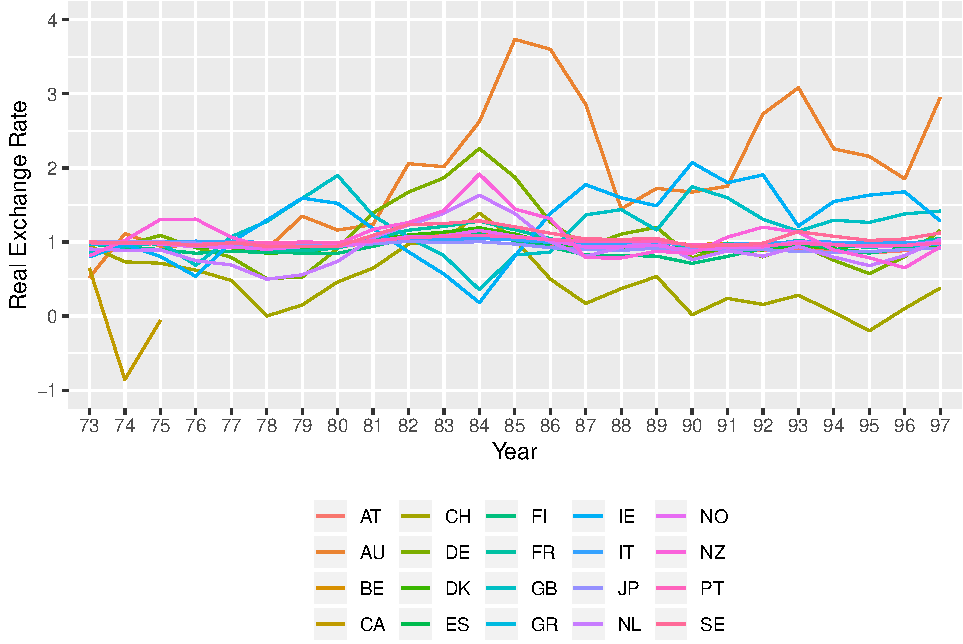
\includegraphics[width=0.75\linewidth]{Time_Series_v_pdf_files/figure-latex/rer2-1} 

}

\caption{Average Year Real Exchange Rate}\label{fig:rer2}
\end{figure}

\hypertarget{results}{%
\subsection{Results}\label{results}}

Following Wu \& Wu (2001), we applied the recursive t-test procedure proposed by Campbell and Perron (1991) to determine the lag order for each country, since this procedure has better size and power than AIC and SBC criterion. Basically, it starts with a model with a big number of lags (\(k_{max}\)) and then the lags should be dropped off the equation if they are not significant. Wu \& Wu (2001) started with \(k_{max}=24\), but here we chose to start with \(k_{max}=12\) and used the 10\% value of the asymptotic normal distribution to determine significance.

Table \ref{tab:adf} shows the lag order (selected by the recursive t-test procedure), the coefficient \(\rho\) and its standard deviation, and the ADF Test p-value. The four variables are presented for each country. Although the results are not exactly the same than those found by Wu and Wu, the main conclusion remains: In general, it is not possible to reject the null non-stationarity hypothesis. As Wu \& Wu, the ADF test cannot reject the unit root null of real exchange rates at the 5 percent. The only exception is New Zealand.

Wu \& Wu also mention in their paper, that one possible reason for the failure of the ADF test to reject the unit root null may be the time span of the data. However, it is possible to exploit cross-section variability among countries applying both, the IPS and Maddala-Wu tests, to examine the unit root null of real exchange rates.

For panel unit roots tests, we only replicate the case with general serial correlation (we discard the homogeneous assumption on the order of serial correlation). The results are shown in Table \ref{tab:purt}. Like Wu \& Wu (2001), we found evidence to reject the unit root hypothesis for both, IPS and Maddala-Wu tests. Even more, we found stronger evidence than what Wu \& Wu did.

The IPS test rejects non-stationarity for the full sample group and the EC group at 1\%,and at 5\% for the other subsamples, while the MW test rejects non-stationarity for the full sample group and the EC group at 5\%, and at 10\% for the other subsamples.

\hypertarget{general-conclusions}{%
\section{General Conclusions}\label{general-conclusions}}

The results obtained and presented in this paper through replications of two well-known papers in the Purchasing Power Parity theory, reaffirm the ambiguous views that economists hold about this concept. Its is unclear whether the PPP holds or, if it does, how long does it take.

Current studies that have reached to reject the random walk hypothesis using unit root tests, estimate a convergence ranging between 3 to 5 years, which results in a issue when collecting data. In this line, panel data tests have provided a handy solution to the problem and the Wu \& Wu 2001 paper is able to show significant differences between the results obtained with both methods.

However, some important cautions must be taken into account when using panel data tests, in particular, regarding the countries that are included in the sample. One of the main critics made to this tests concern the inclusion of countries that exhibit hyperinflation, whose aggregate price level can converge faster to the PPP levels making the null hypothesis easier to reject.

Given the results obtained here and through out time, it is very likely that the PPP actually holds, but the low power of unit root and cointegration tests is one of the main causes for the difficulty to prove this hypothesis, since importantly large samples are needed. Nevertheless, it is not correct to discard the fact that the PPP may be just have a very slow mean reversal, specially for those currencies that are subject to relatively frequently strong shocks due to the country instability.

If PPP should still be used as a reliable reference of exchange rate economic policies, right now, this remains as a question without a definite answer and subject to each country's criteria.

\hypertarget{appendix}{%
\section{Appendix}\label{appendix}}

\listoftables

\begin{table}

\caption{\label{tab:ner}Testing null-hypothesis of I(1) in the nominal exchange rate}
\centering
\begin{tabular}[t]{lcc}
\toprule
Country & ADF p-value of series & ADF p-value of first differences\\
\midrule
UK & 0.63 & < 0.01\\
Germany & 0.71 & < 0.01\\
France & 0.57 & < 0.01\\
Canada & 0.13 & < 0.01\\
Japan & 0.41 & < 0.01\\
\bottomrule
\end{tabular}
\end{table}

\begin{table}

\caption{\label{tab:pl}Testing null-hypothesis of I(1) in the relative price levels}
\centering
\begin{tabular}[t]{lcc}
\toprule
Country & ADF p-value of series & ADF p-value of first differences\\
\midrule
UK & 0.61 & < 0.01\\
Germany & 0.96 & < 0.01\\
France & 0.89 & 0.02\\
Canada & 0.57 & 0.03\\
Japan & < 0.01 & 0.05\\
\bottomrule
\end{tabular}
\end{table}

\begin{table}

\caption{\label{tab:coin}Cointegration regressions}
\centering
\begin{tabular}[t]{lccccc}
\toprule
Country & Constant & $\beta$ & $R^2$ & ADF p-value of reg residuals & EGCM test\\
\midrule
UK & 0.48 & 0.92 & 0.44 & 0.70 & Not cointegrated\\
Germany & -0.90 & -0.10 & < 0.01 & 0.71 & Not cointegrated\\
France & -1.57 & 2.63 & 0.80 & 0.49 & Not cointegrated\\
Canada & -0.04 & 2.37 & 0.60 & 0.64 & Not cointegrated\\
Japan & -5.16 & 0.48 & 0.14 & 0.45 & Not cointegrated\\
\bottomrule
\end{tabular}
\end{table}

\begin{table}

\caption{\label{tab:ner2}Testing null-hypothesis of I(1) in the nominal exchange rate for 1973 - 1998}
\centering
\begin{tabular}[t]{lcc}
\toprule
Country & ADF p-value of series & ADF p-value of first differences\\
\midrule
UK & 0.50 & < 0.01\\
Germany & 0.61 & < 0.01\\
France & 0.72 & < 0.01\\
Canada & 0.82 & < 0.01\\
Japan & 0.50 & < 0.01\\
\bottomrule
\end{tabular}
\end{table}

\begin{table}

\caption{\label{tab:pl2}Testing null-hypothesis of I(1) in the relative price levels for 1973 - 1998}
\centering
\begin{tabular}[t]{lcc}
\toprule
Country & ADF p-value of series & ADF p-value of first differences\\
\midrule
UK & < 0.01 & < 0.01\\
Germany & 0.91 & < 0.01\\
France & 0.96 & < 0.01\\
Canada & 0.97 & < 0.01\\
Japan & 0.06 & < 0.01\\
\bottomrule
\end{tabular}
\end{table}

\begin{table}

\caption{\label{tab:coin2}Cointegration regressions for 1973 - 1998}
\centering
\begin{tabular}[t]{lccccc}
\toprule
Country & Constant & $\beta$ & $R^2$ & ADF p-value of reg residuals & EGCM test\\
\midrule
UK & 0.52 & 0.76 & 0.46 & 0.44 & Not cointegrated\\
Germany & -0.45 & 0.85 & 0.41 & 0.68 & Not cointegrated\\
France & -1.54 & 1.67 & 0.54 & 0.50 & Not cointegrated\\
Canada & -0.11 & 1.27 & 0.23 & 0.97 & Not cointegrated\\
Japan & -4.06 & 1.92 & 0.79 & 0.46 & Not cointegrated\\
\bottomrule
\end{tabular}
\end{table}

\begin{table}

\caption{\label{tab:adf}ADF Tests}
\centering
\begin{tabular}[t]{lcccc}
\toprule
Country & Lag Order & $\rho$ & SE & p-value\\
\midrule
Austria & 3 & -0.071 & 0.03 & 0.398\\
Australia & 3 & -0.068 & 0.033 & 0.361\\
Belgium & 3 & -0.061 & 0.027 & 0.453\\
Canada & 4 & -0.03 & 0.019 & 0.595\\
Switzerland & 3 & -0.087 & 0.034 & 0.257\\
Germany & 3 & -0.07 & 0.03 & 0.446\\
Denmark & 3 & -0.07 & 0.03 & 0.458\\
Spain & 1 & -0.048 & 0.025 & 0.623\\
Finland & 3 & -0.093 & 0.035 & 0.331\\
France & 1 & -0.07 & 0.031 & 0.466\\
Britain & 6 & -0.118 & 0.047 & 0.318\\
Greece & 4 & -0.07 & 0.031 & 0.439\\
Ireland & 3 & -0.109 & 0.04 & 0.185\\
Italy & 3 & -0.081 & 0.034 & 0.381\\
Japan & 1 & -0.039 & 0.022 & 0.481\\
Netherlands & 3 & -0.077 & 0.033 & 0.422\\
Norway & 7 & -0.101 & 0.041 & 0.376\\
New Zealand & 8 & -0.137 & 0.042 & 0.041\\
Portugal & 3 & -0.04 & 0.025 & 0.691\\
Sweden & 7 & -0.083 & 0.031 & 0.309\\
\bottomrule
\end{tabular}
\end{table}

\begin{table}

\caption{\label{tab:purt}Panel Unit Roots Tests}
\centering
\begin{tabular}[t]{lcc}
\toprule
Sample & IPS & MW\\
\midrule
All 20 & 0.001 & 0.024\\
EC & 0.009 & 0.045\\
EMS & 0.012 & 0.063\\
G6 & 0.037 & 0.101\\
G10 & 0.018 & 0.073\\
\bottomrule
\end{tabular}
\end{table}

\hypertarget{references}{%
\section{References}\label{references}}

\begin{itemize}
\item
  Abuaf, N., \& Jorion, P. (1990). ``Purchasing Power Parity in the Long Run''. The Journal of Finance, 45(1), 157-174.
\item
  Adler, M. and Lehmann, B. (1983), ``Deviations from Purchasing Power Parity in the Long Run''. The Journal of Finance, 38: 1471-1487.
\item
  Bowman, David (1999). ``Efficient Tests for Autoregressive Unit Roots in Panel Data''. Manuscript, Federal Reserve Board.
\item
  Breuer, J. B., McNown, R. and Wallace, M. (2002), ``Series?specific Unit Root Tests with Panel Data''. Oxford Bulletin of Economics and Statistics, 64: 527-546.
\item
  Dickey, D., \& Fuller, W. (1979). ``Distribution of the Estimators for Autoregressive Time Series With a Unit Root''. Journal of the American Statistical Association, 74(366), 427-431.
\item
  Engle, R., \& Granger, C. (1987). ``Co-Integration and Error Correction: Representation, Estimation, and Testing''. Econometrica, 55(2), 251-276.
\item
  Frankel, J., \& Froot, K. (1990). ``Chartists, Fundamentalists, and Trading in the Foreign Exchange Market''. The American Economic Review, 80(2), 181-185.
\item
  Frankel, J., Rose, A. (1995). ``Chapter 33 Empirical research on nominal exchange rates'', In \emph{Handbook of International Economics}, Elsevier, Volume 3, 1995, pp.~1689-1729.
\item
  Hakkio, C., (1984). ``A re-examination of purchasing power parity: A multi-country and multi-period study'', Journal of International Economics,17(3?4), 265-277.
\item
  Hoang N.T., McNown R.F., (2006) ``Panel Data Unit Roots Tests Using Various Estimation Methods''. Department of Economics - University of Colorado at Boulder.
\item
  Jorion, P. \& Sweeney, R.J. (1996). ``Mean reversion in real exchange rates: evidence and implications for forecasting'', Journal of International Money and Finance, 15(4), 535-550.
\item
  Kugler, P., \& Lenz, C. (1993). ``Multivariate Cointegration Analysis and the Long-Run Validity of PPP''. The Review of Economics and Statistics, 75(1)
\item
  Levin, A., Chien-Fu Lin, Chia-Shang James Chu (2002). ``Unit root tests in panel data: asymptotic and finite-sample properties'', Journal of Econometrics, 108(1), 1-24.
\item
  Levin, A. and Lin, C. F. (1992). ``Unit Root Test in Panel Data: Asymptotic and Finite Sample Properties'', University of California at San Diego, Discussion Paper No.~92-93.
\item
  Lothian, J., \& Taylor, M. (1996). ``Real Exchange Rate Behavior: The Recent Float from the Perspective of the Past Two Centuries''. Journal of Political Economy, 104(3), 488-509.
\item
  Maddala, G. S. and Wu, S. (1999), A Comparative Study of Unit Root Tests with Panel Data and a New Simple Test. Oxford Bulletin of Economics and Statistics, 61: 631-652.
\item
  MacDonald, R. (1996). ``Panel unit root tests and real exchange rates'', Economics Letters, 50(1), 7-11.
\item
  Mark P. Taylor (1988). ``An empirical examination of long-run purchasing power parity using cointegration techniques'', Applied Economics, 20:10, 1369-1381.
\item
  O'Connell, P.G.J. (1998a, 1997). ``The Overvaluation of Purchasing Power Parity''. Journal of International Economics, 44(1), 1?19.
\item
  Oh, Keun-Yeob. (1996). ``Purchasing power parity and unit root tests using panel data''. Journal of International Money and Finance,15(3), 405-418.
\item
  Papell, David and Theodoridis, Hristos. (2001). ``The Choice of Numeraire Currency in Panel Tests of Purchasing Power Parity''. Journal of Money, Credit and Banking, 33(3), pp.~790-803.
\item
  Papell, David H. (2002). ``The great appreciation, the great depreciation, and the purchasing power parity hypothesis,'' Journal of International Economics, Elsevier, vol.~57(1), 51-82.
\item
  Papell, D.H. (2006). ``The Panel Purchasing Power Parity Puzzle'', Journal of Money, Credit y Banking, 38: 447-467.
\item
  Papell, D.H., Theodoridis, H. (1998). ``Increasing evidence of purchasing power parity over the current float'', Journal of International Money and Finance, 17(1), 41-50.
\item
  Perron, P. (1989). ``The Great Crash, the Oil Price Shock, and the Unit Root Hypothesis''. Econometrica, 57(6), 1361-1401.
\item
  Rogalski, R.,\& Vinso, J. (1977). ``Stock Returns, Money Supply and the Direction of Causality''. The Journal of Finance, 32(4), 1017-1030.
\item
  Rogoff, K. (1996). The Purchasing Power Parity Puzzle. Journal of Economic Literature, 34(2), 647-668.
\item
  Roll, R. (1979). ``Violations of Purchasing Power Parity and Their Implications for International Commodity Markets''. In \emph{International Finance and Trade}, Sarnat, M. and G. P. Szego, Vol. I, Cambridge, MA: Ballinger Publishing Company, pp.~133-176.
\item
  Summers, R. \& Heston, A. (1991). ``THE PENN WORLD TABLE (MARK 5): AN EXPANDED SET OF INTERNATIONAL COMPARISONS, 1950-1988''. The Quarterly Journal of Economics. 106(2), 327-368.
\item
  Taylor, A. \& Taylor, M. (2004). ``The Purchasing Power Parity Debate'', Journal of Economic Perspectives, 18(4), 135-158.
\item
  Wu, Y. (1996). ``Are Real Exchange Rates Nonstationary? Evidence from a Panel-Data Test''. Journal of Money, Credit and Banking, 28(1), 54-63.
\item
  Wu, J., \& Wu, S. (2001). ``Is Purchasing Power Parity Overvalued?'' Journal of Money, Credit and Banking, 33(3), 804-812.
\end{itemize}

\end{document}
